\subsubsection{Loops: results}\label{sec:loops:results}

\begin{table}[h!]
  \centering
  \begin{tabular}{llll}
    Step-limit parameter $L$ & Nonhalt                         & Halt                           & Total decided \\
    130                      & 126,950,828                     & 48,367,435                     & 175,318,263   \\
    4100                     & 43,269                          & 12,276                         & 55,545        \\
    1,050,000                & 2                               & 0                              & 2             \\ \hline
    Total                    & \multicolumn{1}{r}{126,994,099} & \multicolumn{1}{r}{48,379,711} & 175,373,810
  \end{tabular}
  \caption{5-state machines decided by loops (Algorithm~\ref{alg:loops}) per step-limit parameter $L$.}\label{tab:paramsLoops}
\end{table}

The decider for loops, Algorithm~\ref{alg:loops}, is implemented as part of Coq-BB5 (function \texttt{loop1\_decider}). As advertised in the $S(5)$ pipeline (Table~\ref{tab:pipelineBB5}), it decides a very important proportion the enumerated 5-state Turing machines: 95.48\% of the nonhalting machines and 99.99\% of the halting ones and this with fairly low step-limit parameters, see Table~\ref{tab:paramsLoops}! This means, for instance, that 99.99\% of the enumerated 5-state halting machines halt before $4,100$ steps.

\begin{figure}
  \centering
  % 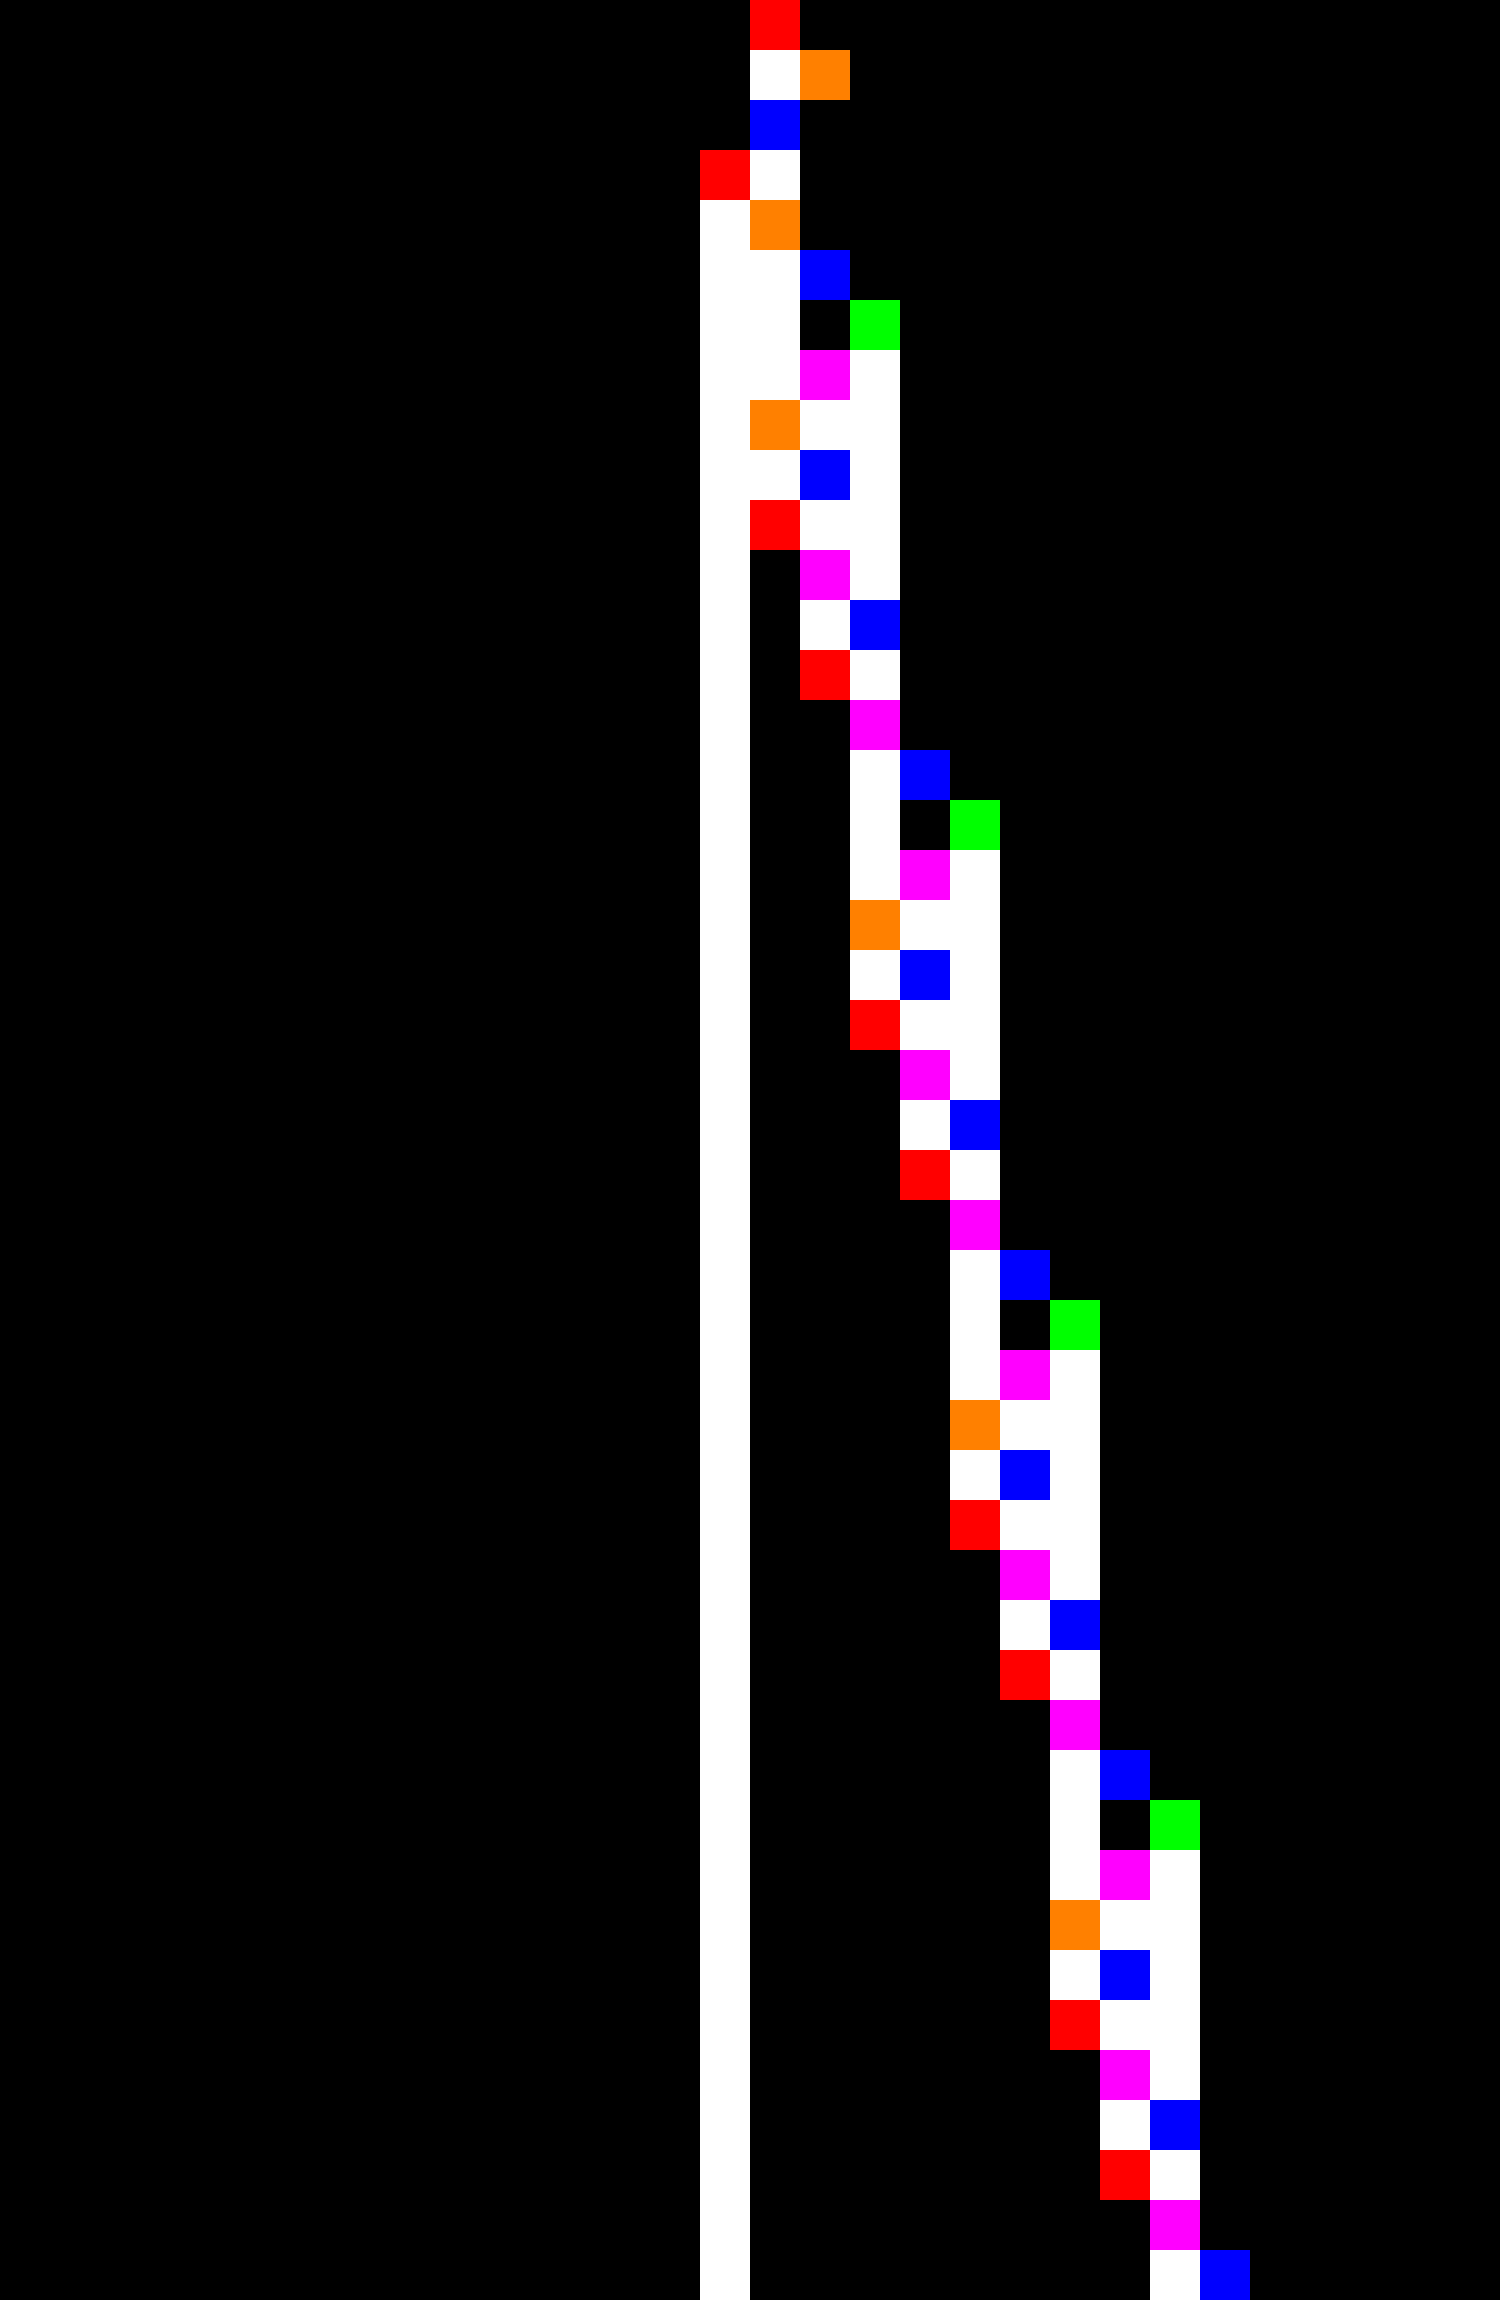
\includegraphics[width=0.5\textwidth]{figures/space-time-diagrams/translated_cycler_44394115.pdf}
  % \hspace{2ex}
  \includegraphics[width=0.5\textwidth]{figures/space-time-diagrams/translated_cycler_59090563.png}

  \caption{10,000-step space-time diagram of a Translated cycler not decided by the decider for loops in \CoqBB (it is decided by NGramCPS, see Section~\ref{sec:n-gramCPS}). See \url{https://bbchallenge.org/1RB0LE_1LC0RD_---1LD_1RE0LA_1LA0RE}.}\label{fig:translated-cyclers-more}
\end{figure}


The number of nonhalting machines decided this decider in \CoqBB (\ie $126{,}994{,}099$, see Table~\ref{tab:paramsLoops}) is a lower bound of the actual number of 5-state loops. Two examples:

\begin{enumerate}
  \item Figure~\ref{fig:translated-cyclers-more} gives a \TC that is decided by the $n$-gram Closed Position Set (NGramCPS) decider, see Section~\ref{sec:n-gramCPS}, this is because higher step-limit $L$ would have been needed to be detected by Algorithm~\ref{alg:loops}.
  \item Infamously, the Sporadic machine (\ie machine which required an individual proof of nonhalting) ``Skelet \#1'', see Section~\ref{sec:sporadic}, is a \TC but with enormous parameters: it does not start looping before $5.42 \times 10^{51}$ steps and has a period of more than 8 billion steps \cite{ShawnSkelet1}. There is no reasonable step-limit $L$ for which this machine would have been decided, neither in fact any of our deciders which could have decided it as they all more or less rely on step-by-step simulation. An individual proof of nonhalting was required \cite{busycoq}.
\end{enumerate}

\ts{TS: I'd like to say that nonetheless, this sample of $126{,}994{,}099$ suggests that there are X times more TCs than cyclers, but I don't have the actual number. I think that X is of order 10.}